%\part{Spezifikation}

\chapter{Browser}
Im Folgenden werden die verschiedenen Anwendungsfälle des \SECH-Browsers übersichtlich vorgestellt. Sie veranschaulichen die für den Benutzer verfügbaren Funktionalitäten des Browsers.

\section{Menüführung}
\begin{figure}[htb]
\centering
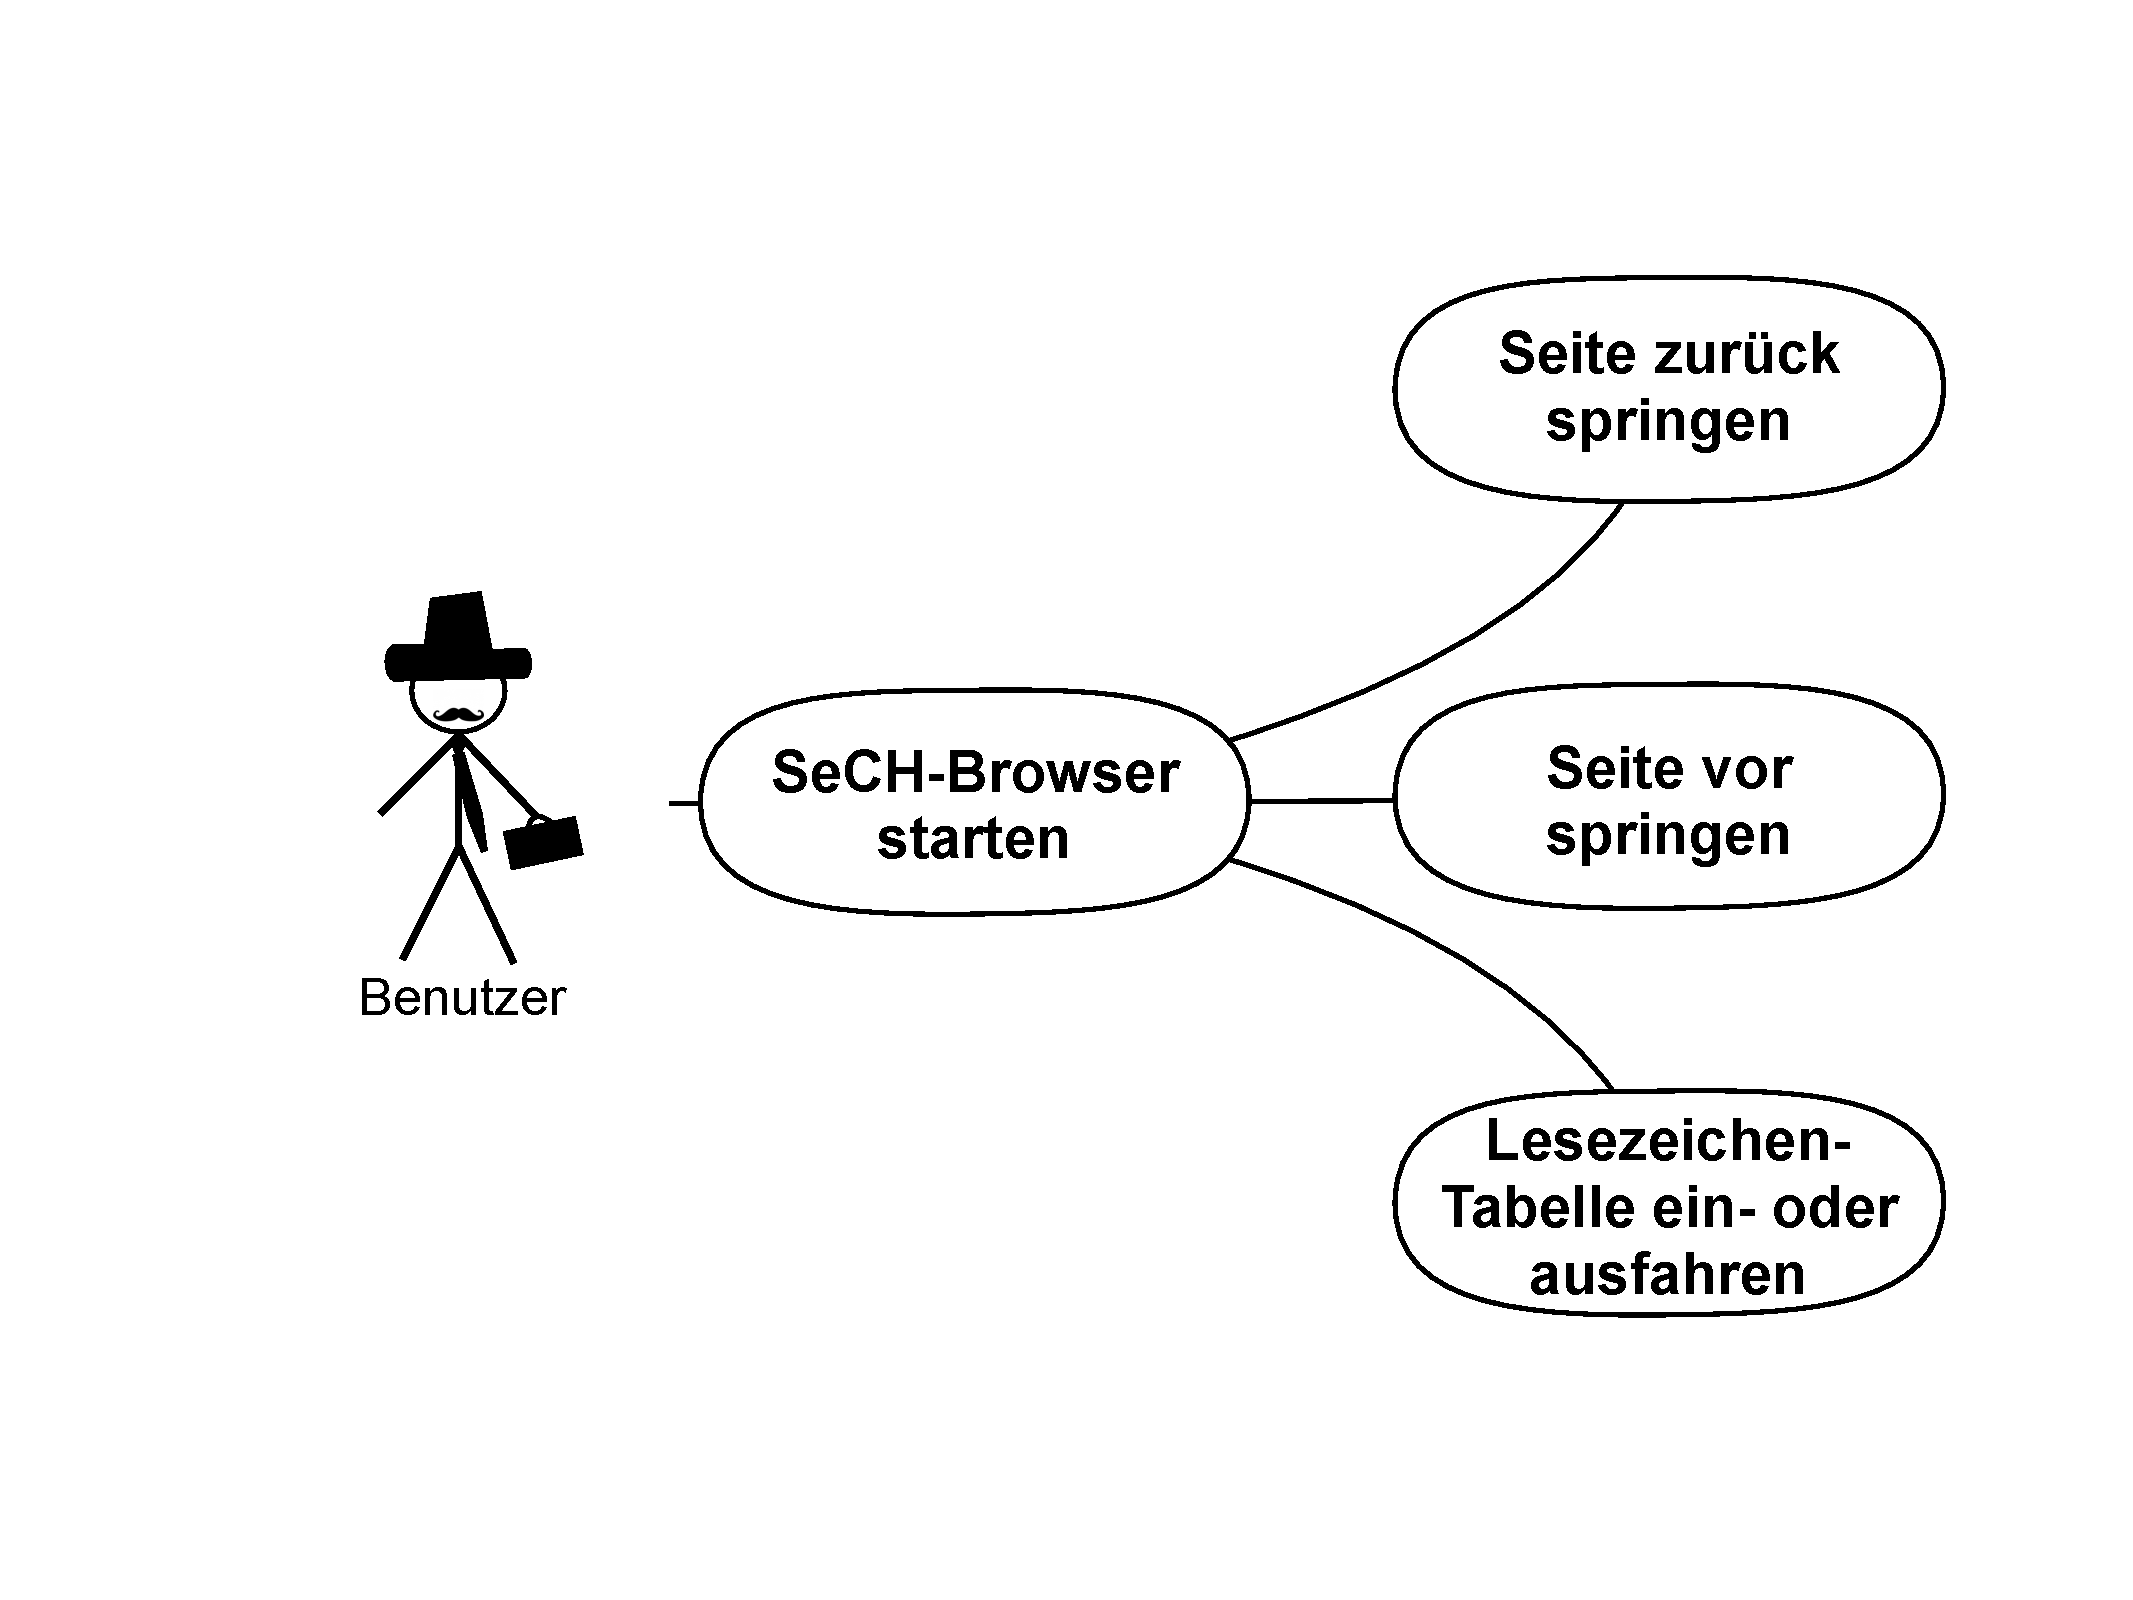
\includegraphics[width=\textwidth]{Use-case-navigieren.pdf}
	\caption{Anwendungsfall \glqq navigieren\grqq\xspace}
\end{figure}
Dieser Anwendungsfall zeigt die wesentlichen Funktionen des Browsers an. Der Nutzer kann auf einer Homepage eine Seite zurück- bzw. wieder vorspringen und er hat die Möglichkeit die Lesezeichentabelle aus- und auch wieder einzufahren.

\begin{figure}[htb]
\centering
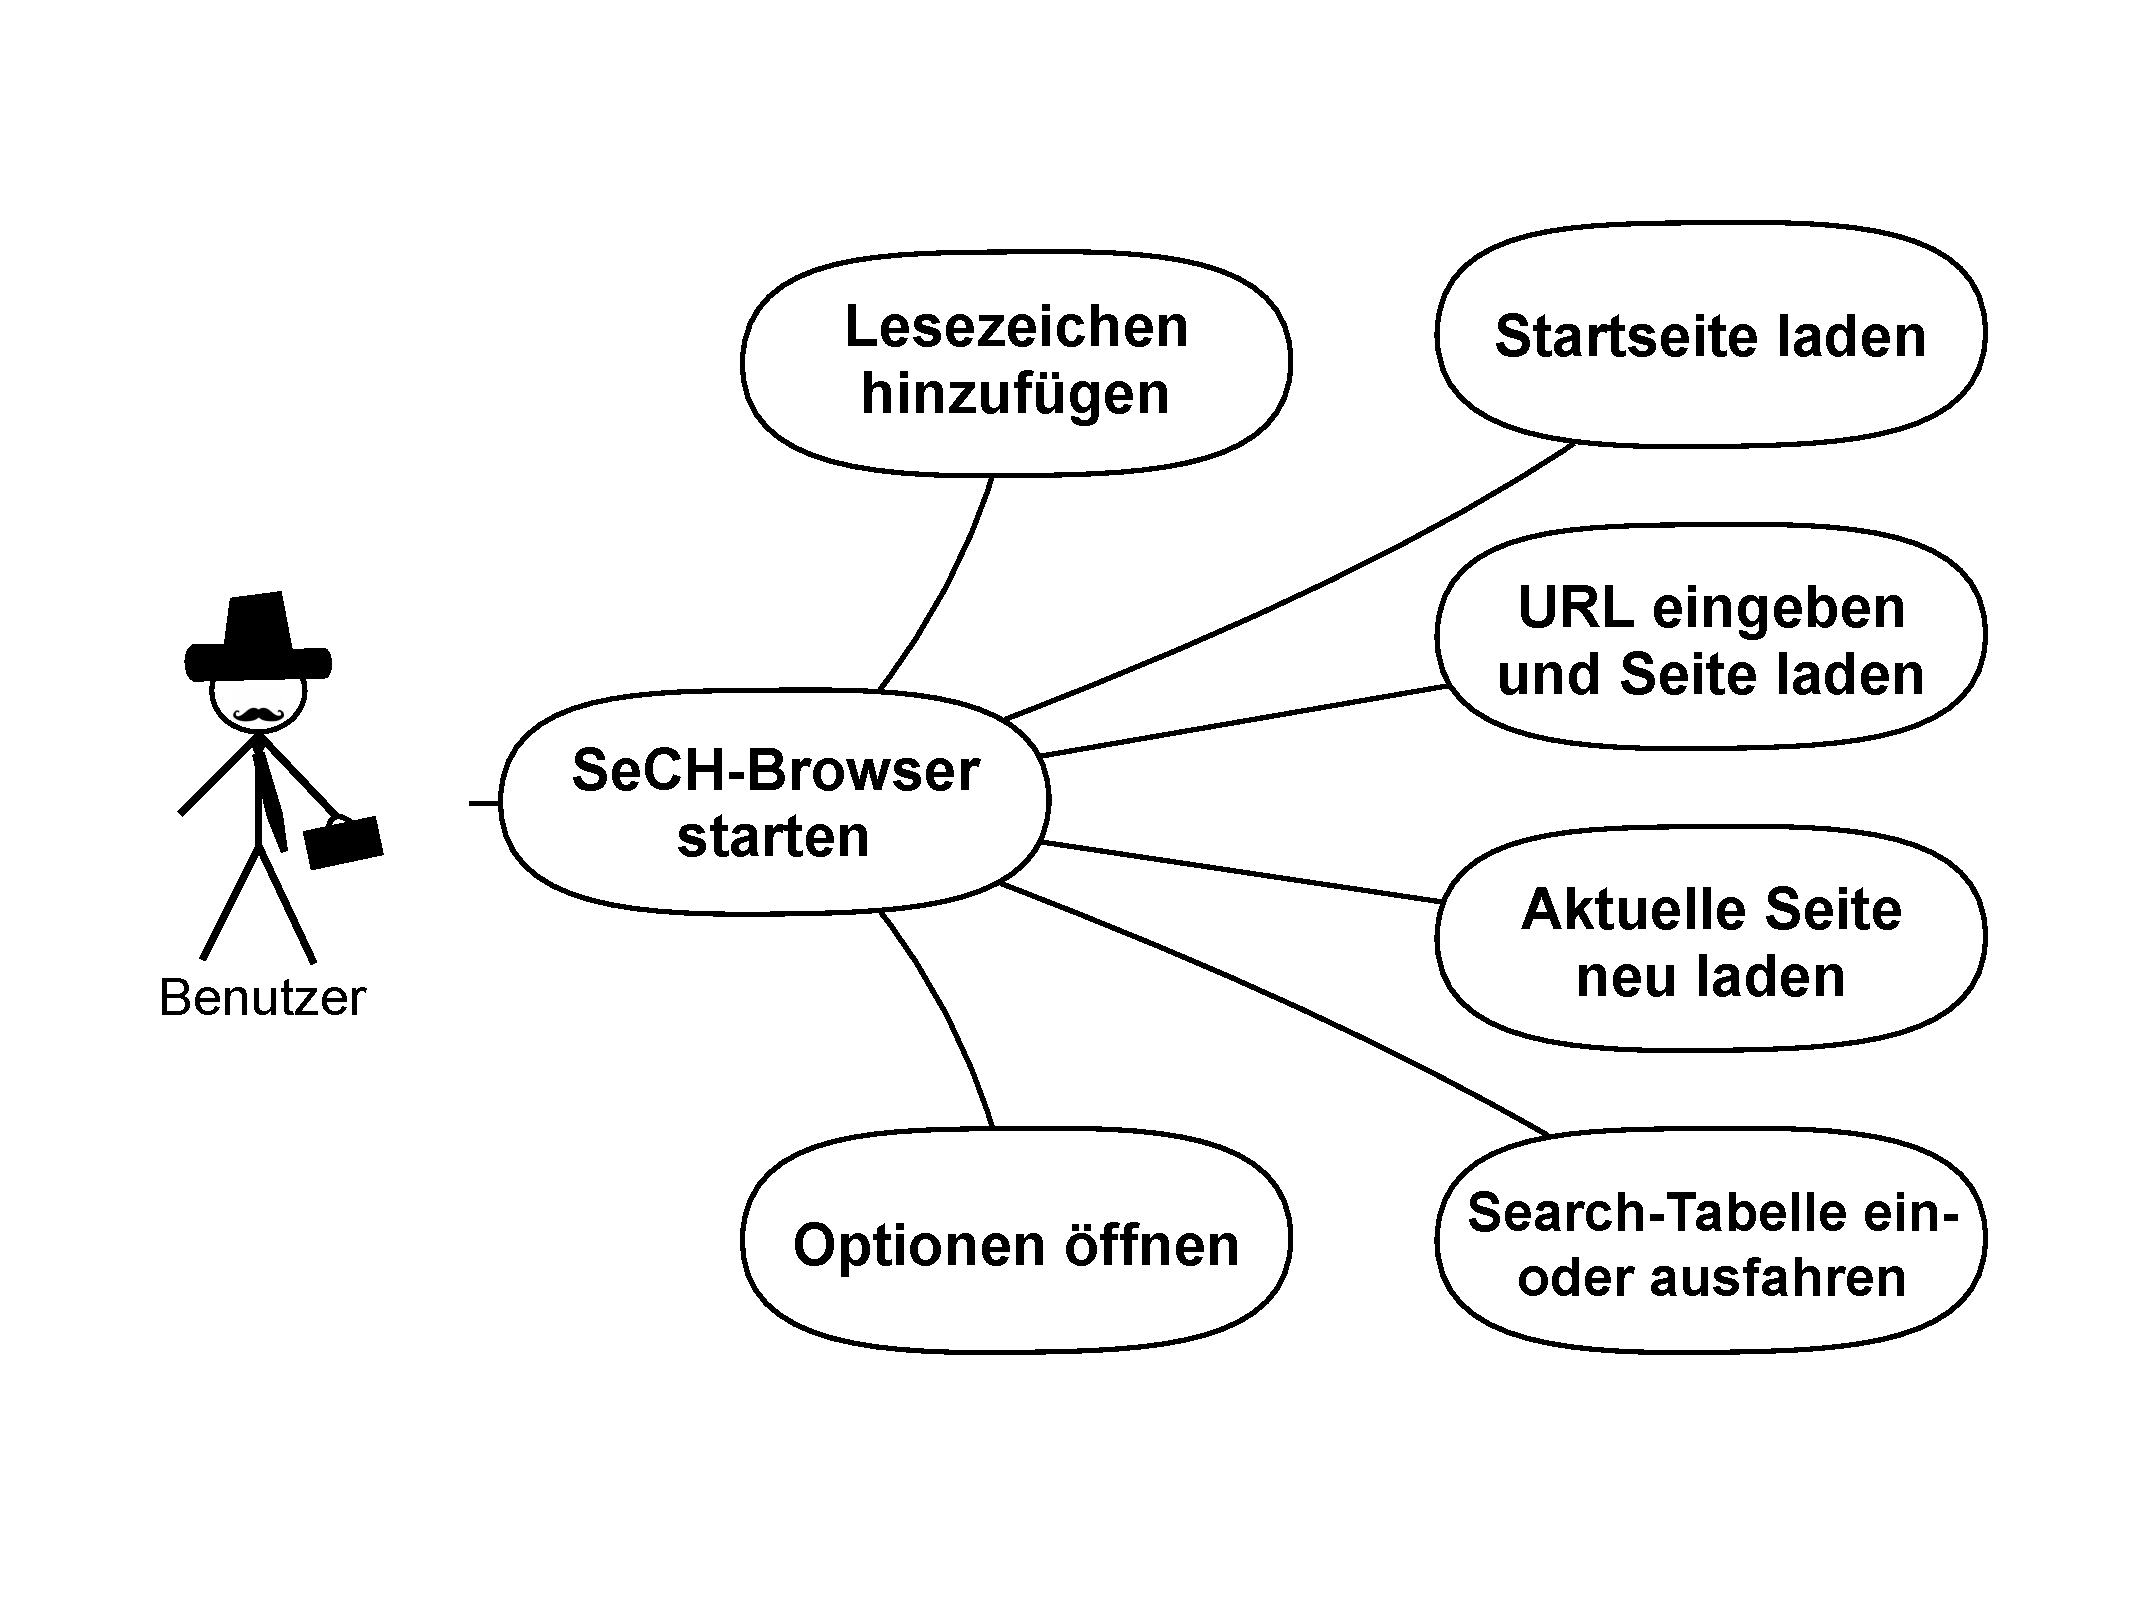
\includegraphics[width=\textwidth]{Use-case-browsen.pdf}
	\caption{Anwendungsfall \glqq browsen\grqq\xspace}
\end{figure}
In diesem Anwendungsfall werden weitere Navigationselemente des Browsers vorgestellt. Der Nutzer kann:
\begin{itemize}
	\item eigene Lesezeichen hinzufügen
	\item die von ihm definierte Startseite laden
	\item eine Webadresse in die Adresszeile eingeben und diese dann aufrufen
	\item die aktuelle Seite neu laden
	\item die \SEARCH-Tabelle aus- und einfahren
	\item das Fenster für Optionen öffnen.
\end{itemize}

\section{Lesezeichenverwaltung}
\begin{figure}[htb]
\centering
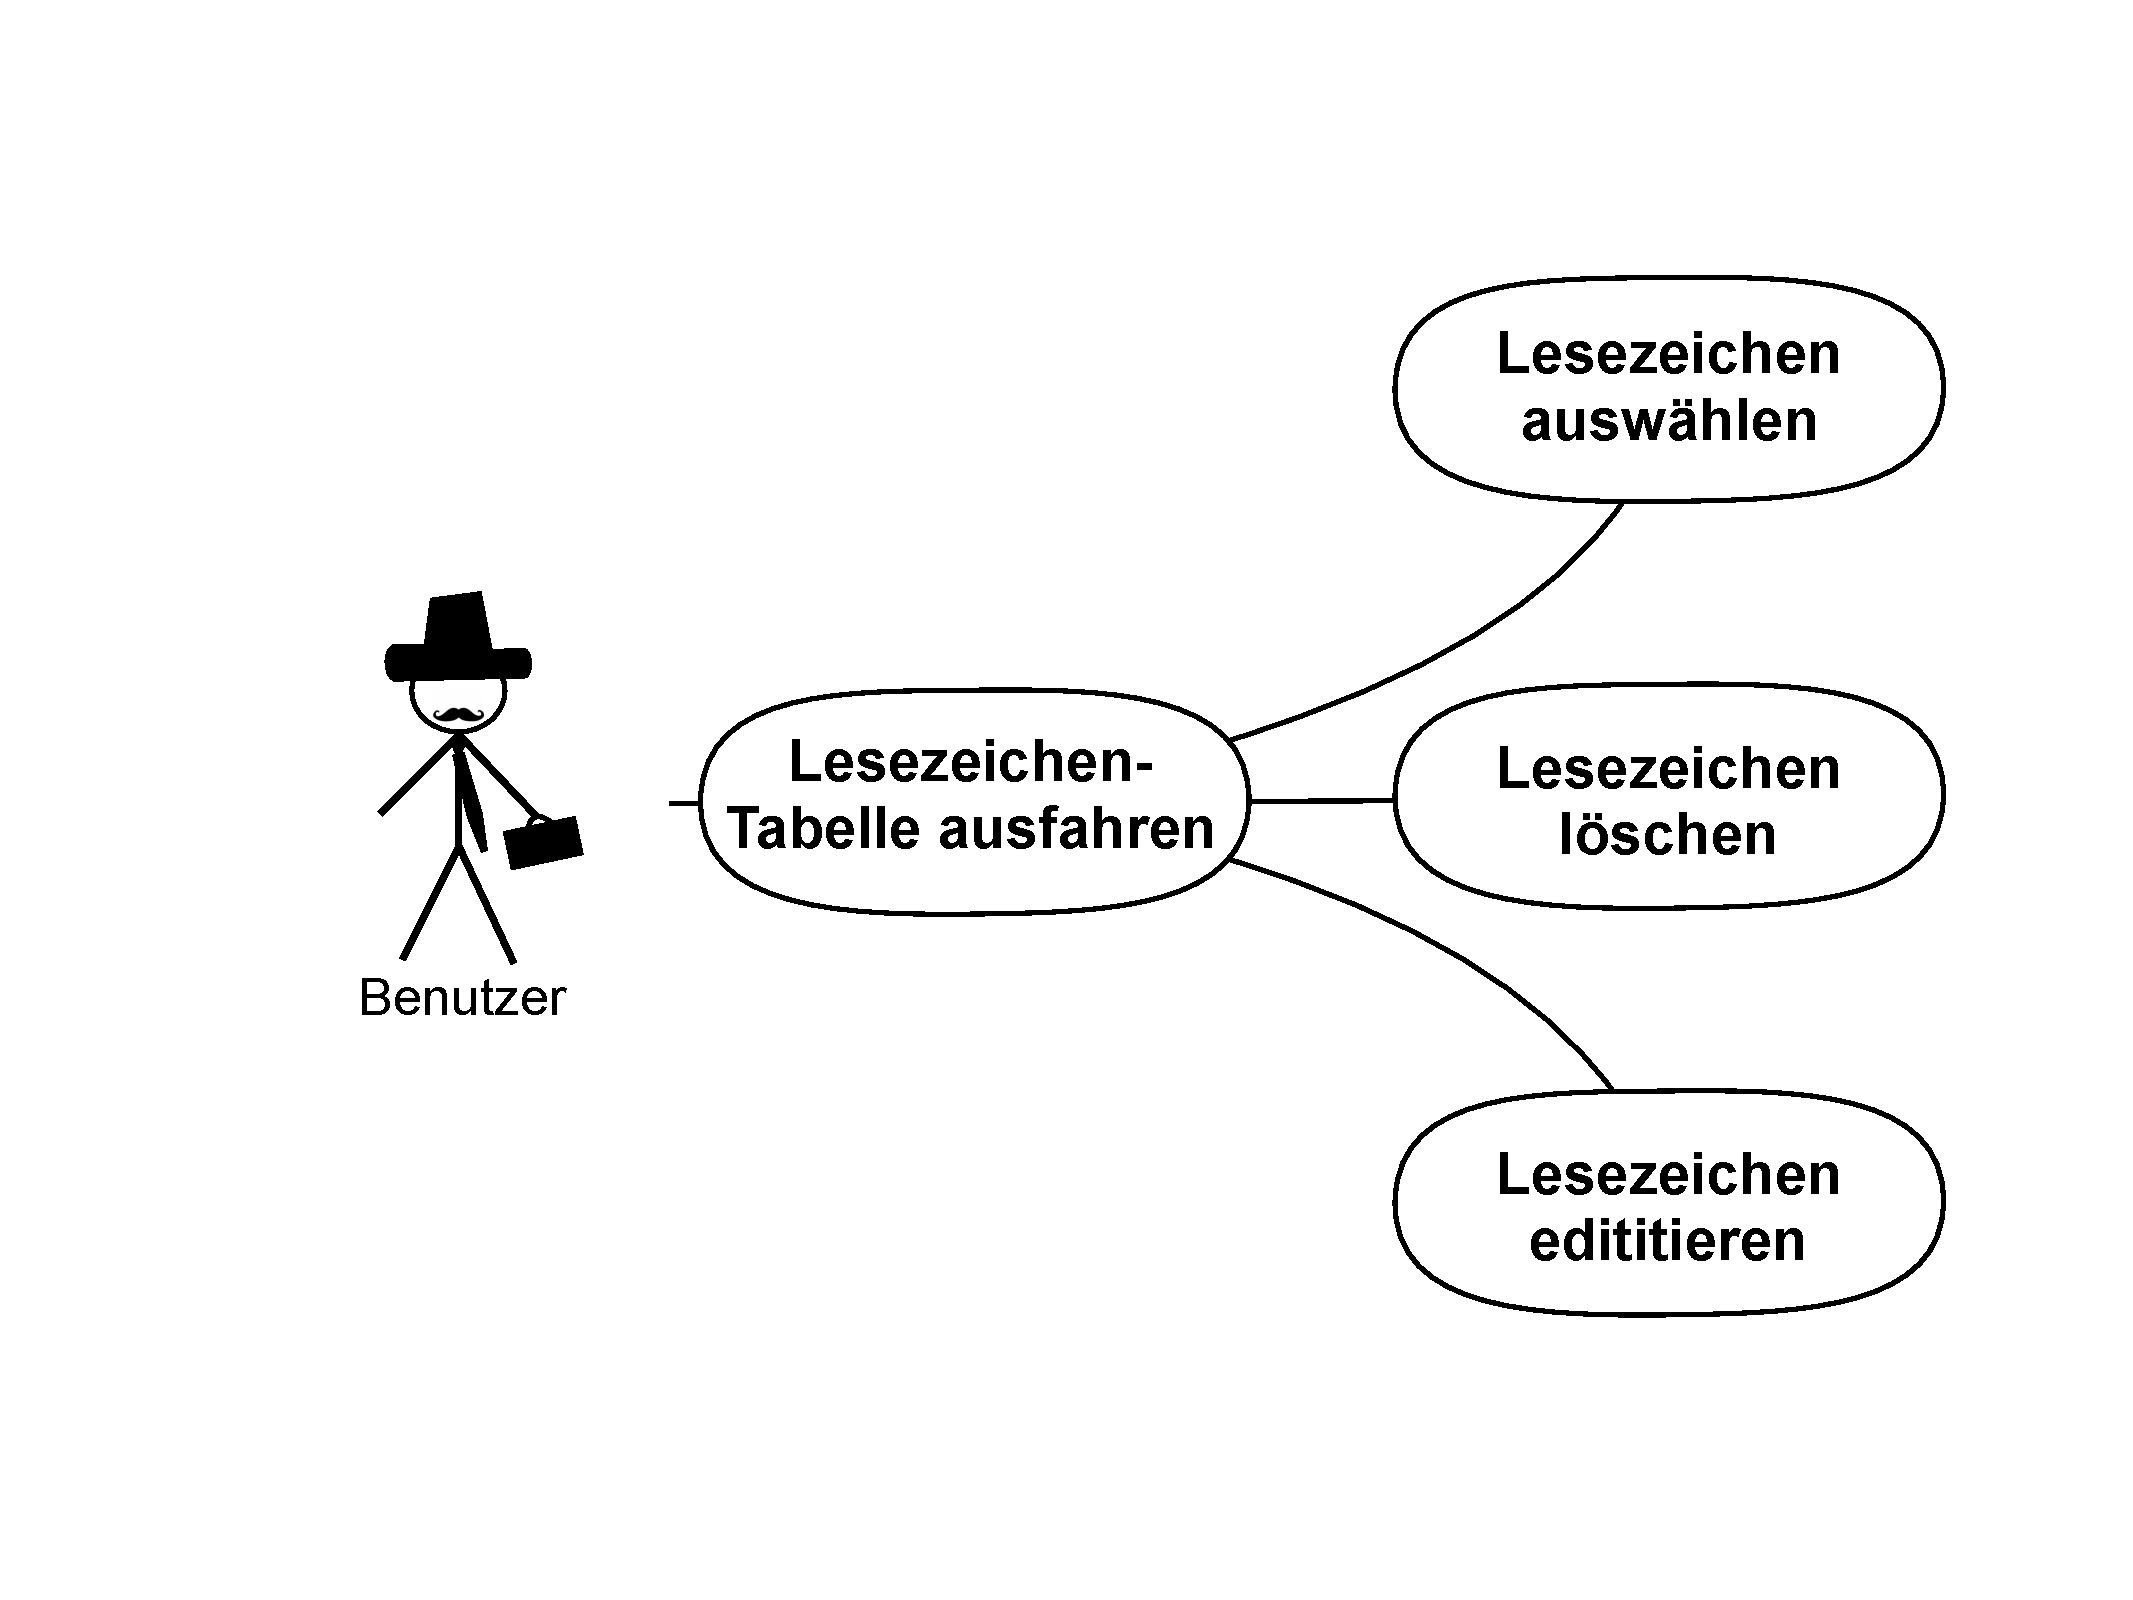
\includegraphics[width=\textwidth]{Use-case-Lesezeichen.pdf} %toDo - SeARCH
	\caption{Anwendungsfall \glqq Lesezeichen\grqq\xspace}
\end{figure}
Ist die Lesezeichentabelle ausgefahren, so kann der Benutzer ein persönlich angelegtes Lesezeichen auswählen und es wird die von ihm gewünschte Seite aufgerufen. Das Löschen und das Editieren ausgewählter Lesezeichen ist ebenfalls in der Tabelle möglich.

\section{\SEARCH-Tagverwaltung}
\begin{figure}[htb]
\centering
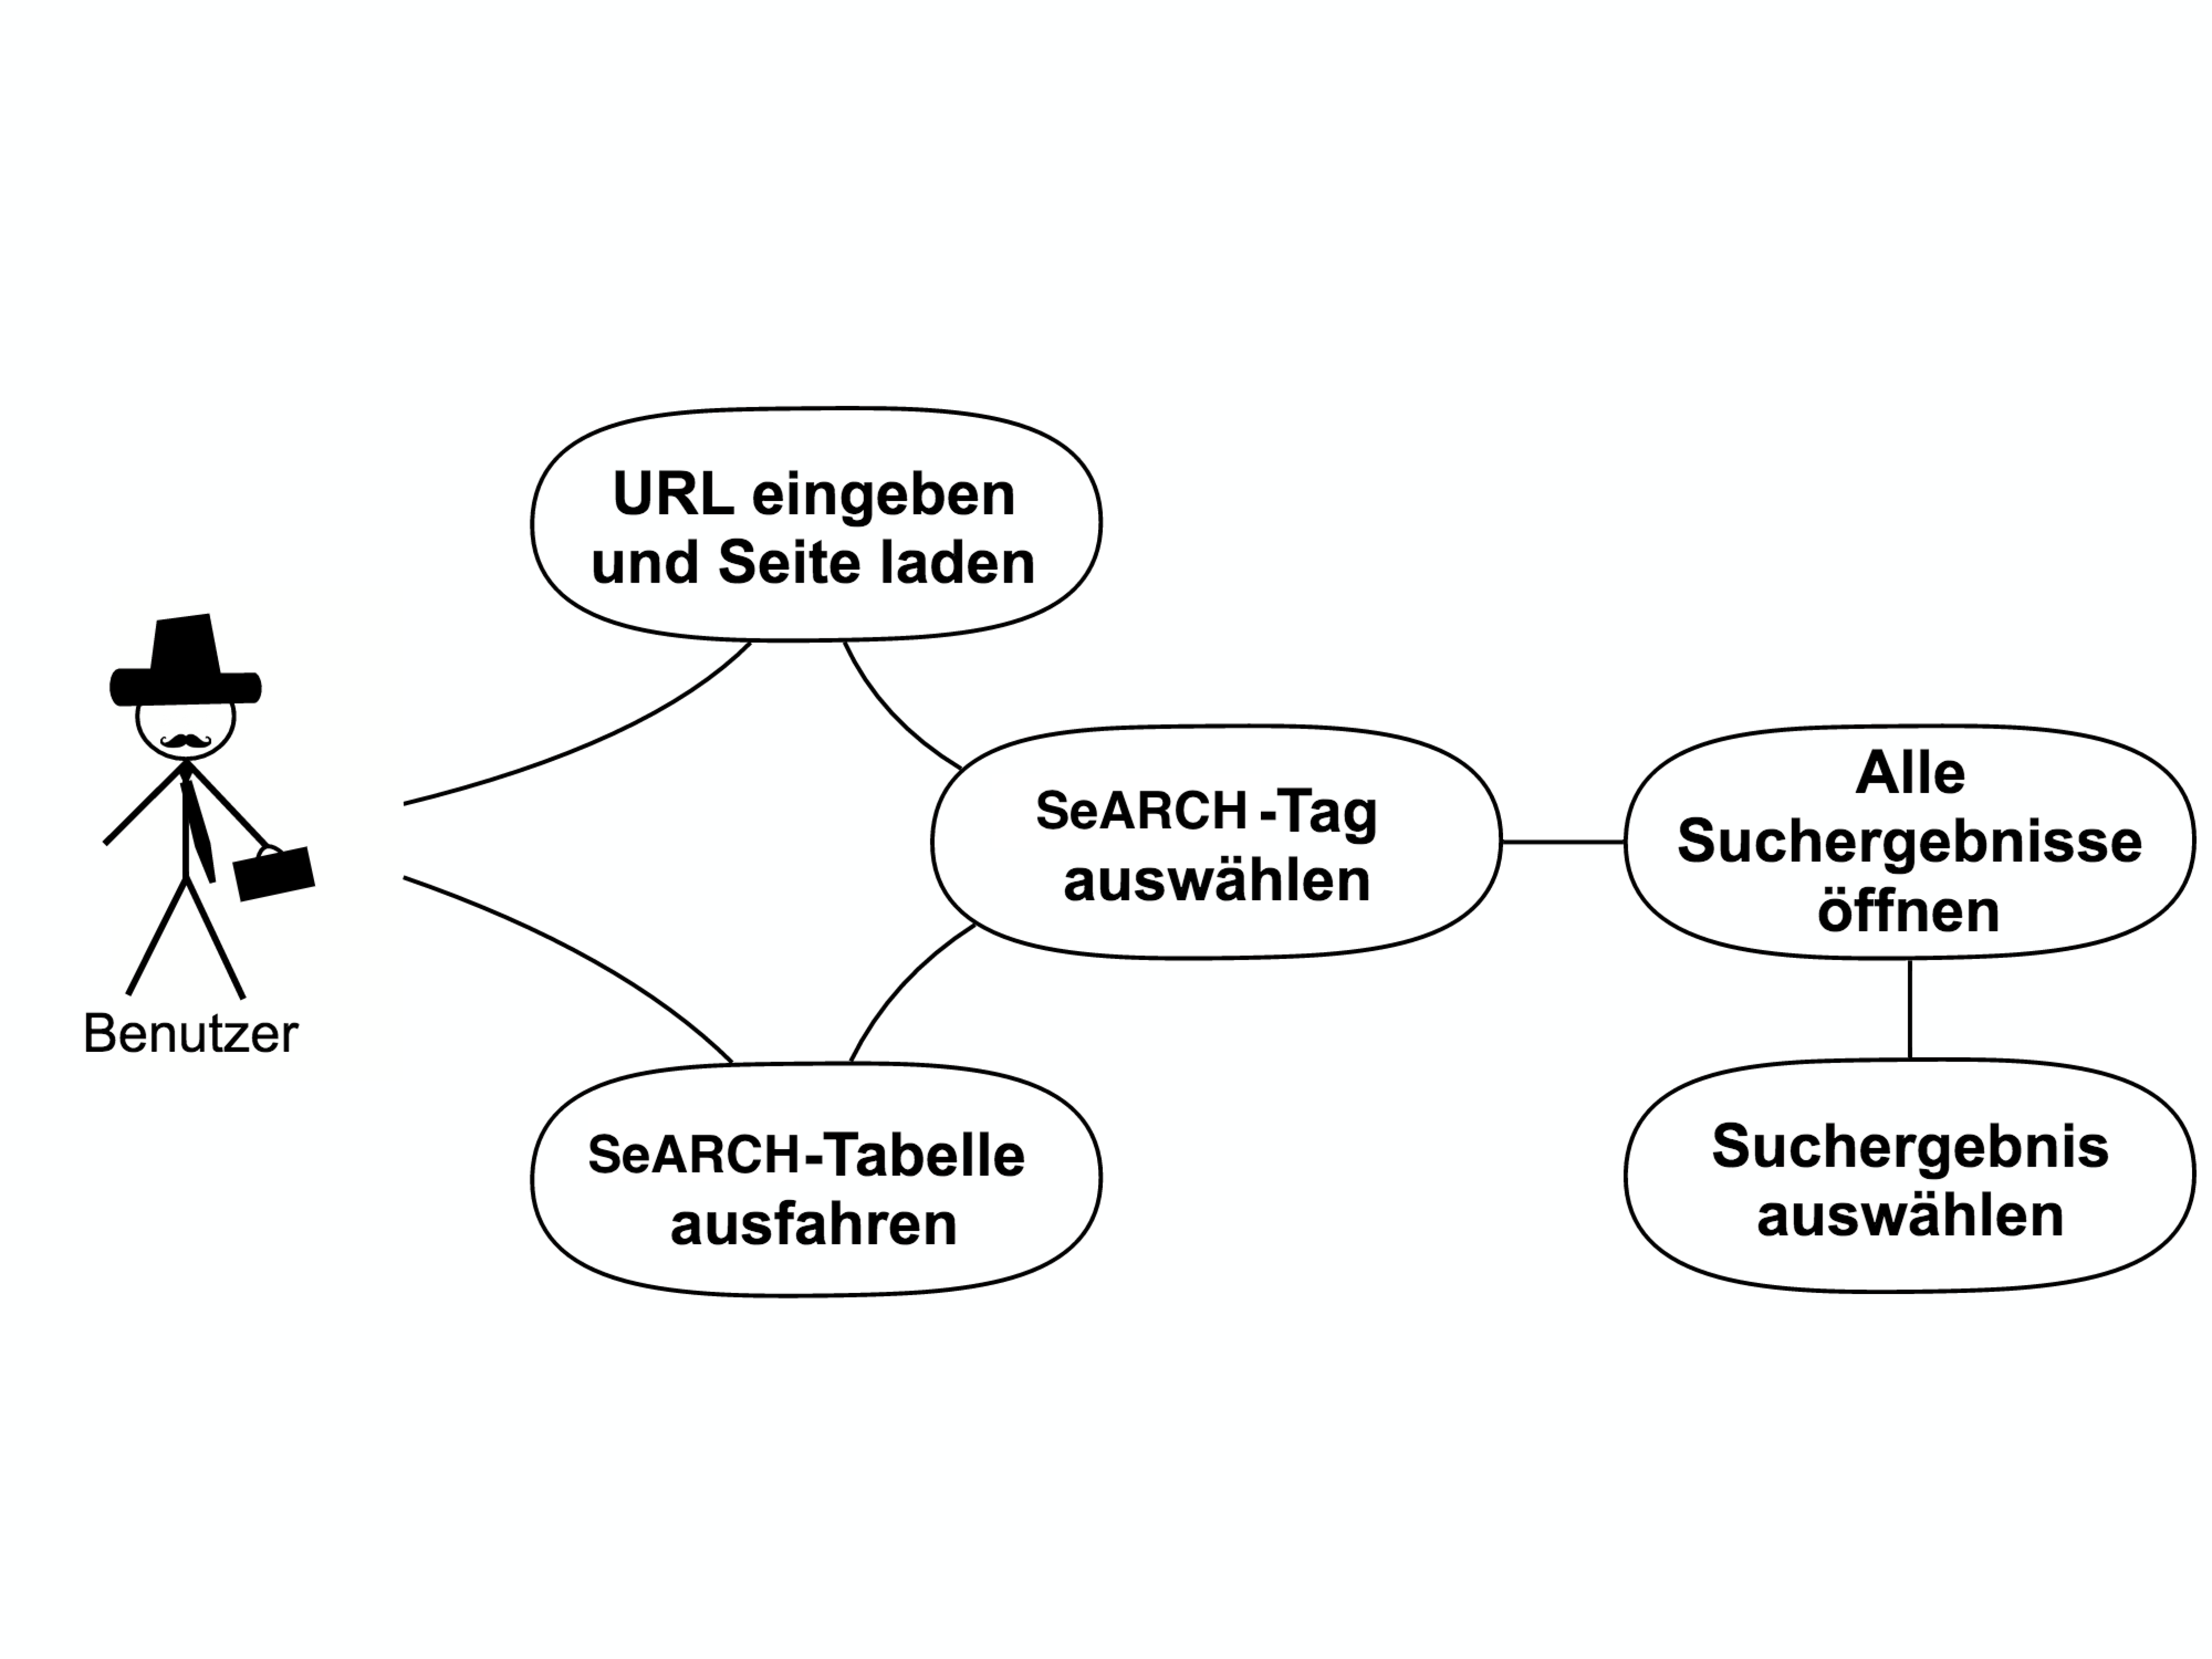
\includegraphics[width=\textwidth]{Use-case-Tagverwaltung.pdf}
	\caption{Anwendungsfall \glqq \SEARCH-Tagverwaltung\grqq}
\end{figure}
Der Nutzer kann sich auf zwei unterschiedlichen Wegen die Suchergebnisse für das gewünschte \SEARCH-Tag anzeigen lassen. Zunächst muss der Nutzer durch Eingabe und Bestätigung einer Webadresse die Seite aufrufen. Die erste Variante ist das hervorgehobene \SEARCH-Tag anzutippen. Alternativ kann der Nutzer in einer zweiten Variante durch Ausfahren der \SEARCH-Tabelle ein gewünschtes \SEARCH-Tag antippen. Beide Wege führen zur Anzeige des ersten Suchergebnisses des jeweiligen \SEARCH-Tags. Anschließend kann der Nutzer sich alle weiteren Suchergebnisse zu einem \SEARCH-Tag anzeigen lassen.
\newpage
\section{Einstellungen}
\begin{figure}[htb]
\centering
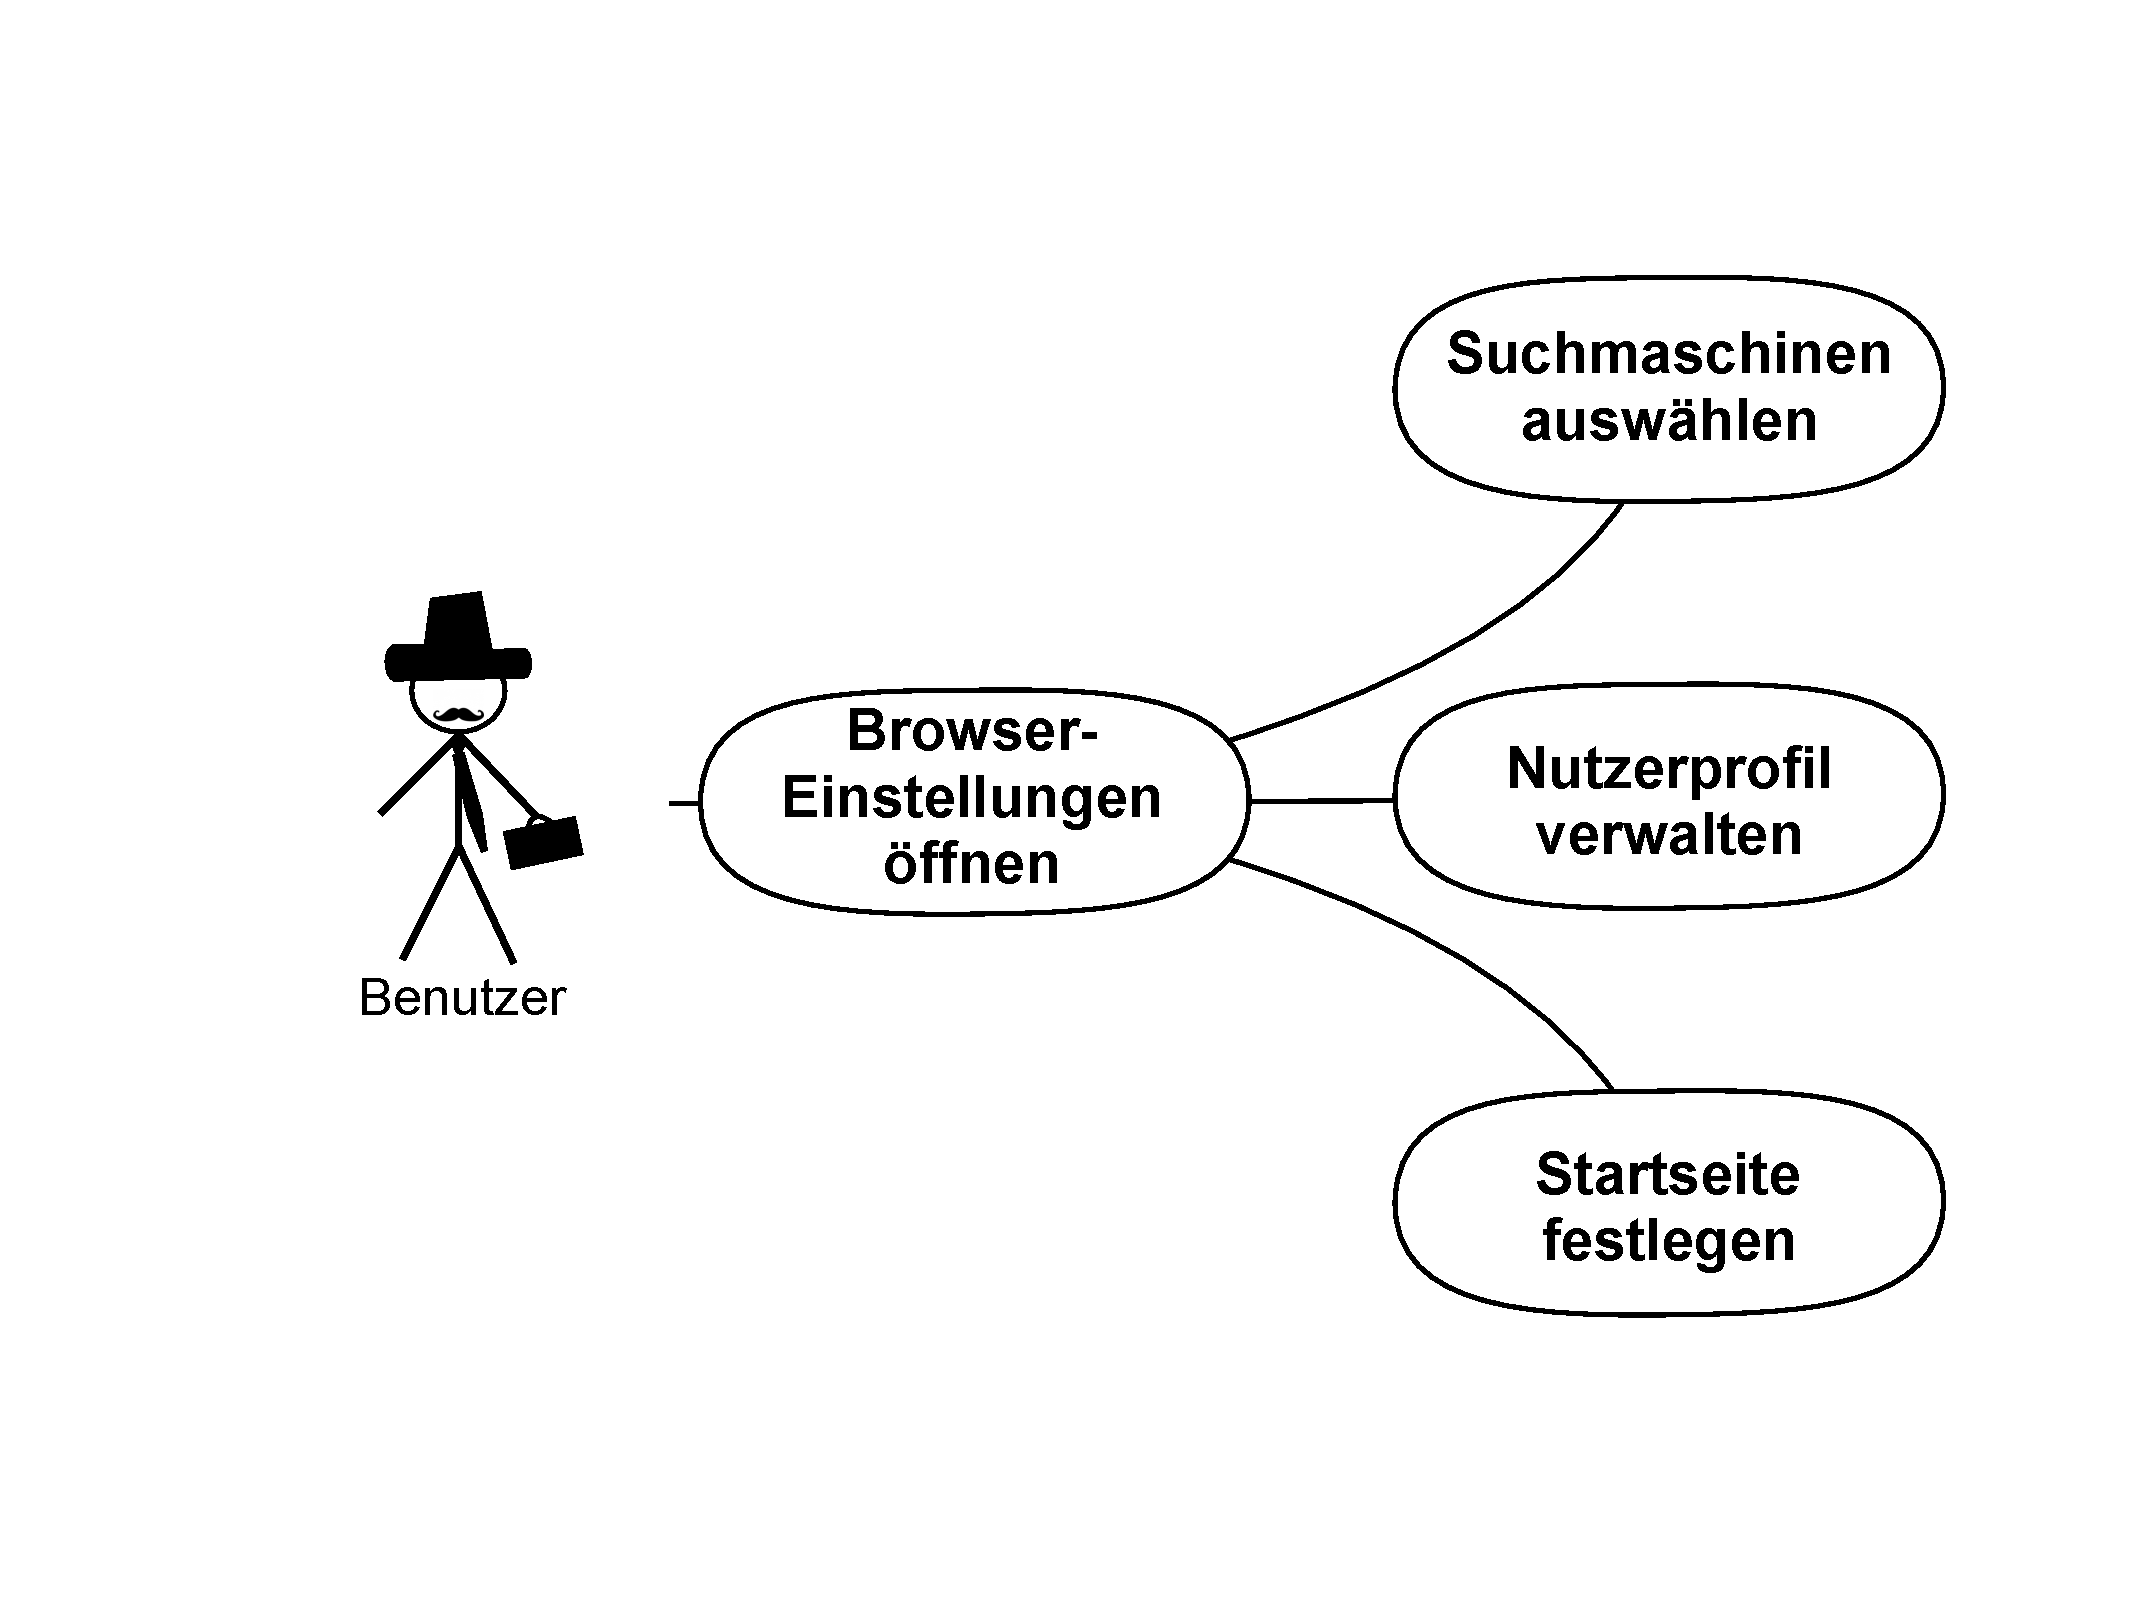
\includegraphics[width=\textwidth]{Use-case-Einstellungen.pdf} %SeARCH
	\caption{Anwendungsfall \glqq Einstellungen\grqq\xspace}
\end{figure}
Befindet sich der Nutzer in den Browsereinstellungen, so hat er die Möglichkeit die Suchmaschinen die für die Suchergebnisse der \SEARCH-Tags verwendet werden sollen auszuwählen. Möchte er bestimmte Suchmaschinen nicht verwenden kann er diese abwählen. Außerdem kann der Benutzer sein persönliches Nutzerprofil verwalten und seine Startseite festlegen, die direkt nach dem Öffnen der Anwendung als erste Seite geladen wird.
